%versi 2 (8-10-2016)
\chapter{Landasan Teori}
\label{chap:teori}

\section{\textit{Linear Programming}}

\textit{Linear programming} adalah sarana untuk menyelesaikan masalah optimasi~\cite{winston2004operations}. Optimasi merupakan usaha untuk memilih solusi terbaik dari suatu kumpulan solusi yang ada. Setiap masalah optimasi perlu diubah terlebih dahulu ke dalam bentuk masalah \textit{linear programming} agar dapat diselesaikan menggunakan \textit{linear programming}. Pada bagian ini, akan dibahas karakteristik dan cara menyelesaikan masalah \textit{linear programming}.

\subsection{Karakteristik}
Masalah \textit{linear programming} memiliki karakteristik sebagai berikut:

\begin{itemize}
	\item \textbf{Variabel keputusan}\\
		Dalam masalah \textit{linear programming}, terdapat variabel keputusan yang mendeskripsikan keputusan yang akan diambil. Contoh:
		
		\begin{equation*}
			\begin{split}
				x_1 &= \text{jumlah produk A yang diproduksi} \\
    			x_2 &= \text{jumlah produk B yang diproduksi}
			\end{split}
		\end{equation*}
		
	\item \textbf{Fungsi Tujuan}\\
		Dalam masalah \textit{linear programming}, terdapat suatu keuntungan yang ingin dimaksimalkan atau suatu kerugian yang ingin diminimalkan dengan menggunakan  fungsi tujuan yang terdiri dari variabel-variabel keputusan. Contoh:
		
		\begin{equation*}
			\textit{max } z = 3x_1 + 2x_2
		\end{equation*}

	\item \textbf{Batasan}\\
		Dalam masalah \textit{linear programming}, terdapat batasan-batasan yang membuat variabel keputusan memiliki nilai yang dibatasi. Batasan juga membuat suatu variabel keputusan berkaitan dengan variabel keputusan lainnya. Contoh:
		
		\begin{equation*}		
			\setlength\arraycolsep{1.5pt}
			\begin{array}{r c r c r}
				2x_1 & + & x_2 & \leq & 100 \\
    			x_1 & + & x_2 & \leq & 80 \\
    			x_1 & & & \leq & 40
			\end{array}
		\end{equation*}
		
	\item \textbf{Batasan non-negatif}\\
		Dalam masalah \textit{linear programming}, batasan non-negatif (\(x_i\geq 0\)) pada variabel keputusan menyatakan bahwa variabel keputusan tersebut tidak dapat bernilai negatif. Dengan batasan non-negatif, variabel keputusan diharuskan untuk bernilai 0 atau positif. Contoh:
		
		\begin{equation*}
			\begin{split}
    			x_1 &\geq 0 \\
    			x_2 &\geq 0
			\end{split}
		\end{equation*}
		
\end{itemize}

Dengan keempat karakteristik di atas, setiap masalah optimasi dapat diubah ke dalam masalah \textit{linear programming} untuk diselesaikan. Berikut contoh masalah \textit{linear programming}:

\begin{equation*}
	\setlength\arraycolsep{1.5pt}
	\begin{array}{r r c r c l}
		\textit{max } &\multicolumn{5}{l}{z = 3x_1 + 2x_2}\\
		\textit{s.t.} &2x_1 &+ &x_2 &\leq &100\\
		&x_1 &+ &x_2 &\leq &80\\
		&x_1 &&&\leq &40\\
		&&&x_1 &\geq &0\\
		&&&x_2 &\geq &0\\
	\end{array}
\end{equation*}

	Tulisan ''\textit{s.t.}'' atau ''\textit{subject to}'' menandakan bahwa nilai dari setiap variabel keputusan harus memenuhi setiap batasan dan batasan non-negatif.

\subsection{Daerah \textit{Feasible} dan Solusi Optimal}
Dalam masalah \textit{linear programming}, terdapat daerah yang bernama daerah \textit{feasible}. Daerah \textit{feasible} dalam suatu masalah \textit{linear programming} merupakan himpunan yang terdiri dari seluruh titik yang memenuhi setiap batasan dan batasan non-negatif~\cite{winston2004operations}. Dengan demikian, setiap titik yang berada di dalam daerah \textit{feasible} merupakan solusi terhadap permasalahan tersebut. Apabila dipilih suatu titik yang berada di luar daerah \textit{feasible}, maka titik ini disebut dengan titik \textit{infeasible}. Titik \textit{infeasible} bukan merupakan solusi bagi permasalahan karena titik ini tidak memenuhi setiap batasan dan batasan non-negatif. Untuk menggambarkan daerah \textit{feasibel}, digunakan contoh batasan-batasan sebagai berikut:

\begin{equation*}
	\begin{array}{r c r c l}		
		2x_1 &+ &x_2 &\leq &100\\
		x_1 &+ &x_2 &\leq &80\\
		x_1 &&&\leq &40\\
		&&x_1 &\geq &0\\
		&&x_2 &\geq &0\\
	\end{array}
\end{equation*}

Pada contoh masalah tersebut, hanya terdapat 2 variabel keputusan sehingga dapat digambarkan dalam diagram kartesius. Pada gambar~\ref{fig:daerah_feasible} terlihat bahwa batasan-batasan membentuk daerah \textit{feasible}.

\begin{figure}[H]
	\centering
	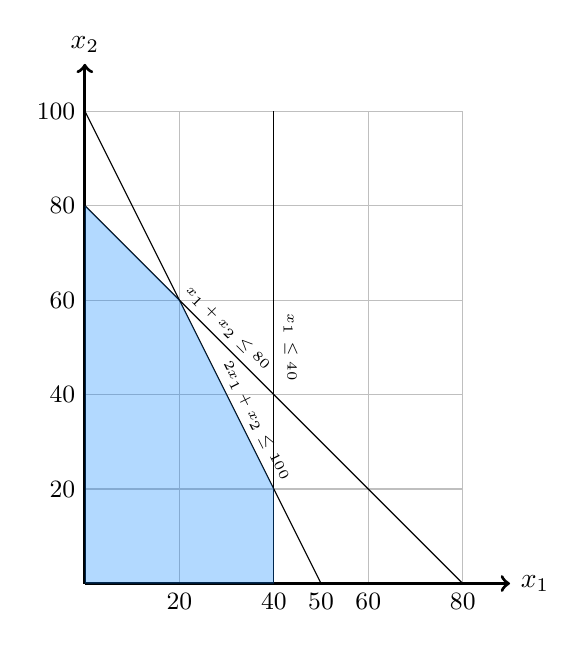
\begin{tikzpicture}[scale=0.06]
		\draw[gray!50, thin, step=20] (0,0) grid (80, 100);
		\draw[very thick,->] (0,0) -- (90, 0) node[right] {$x_1$};
		\draw[very thick,->] (0,0) -- (0, 110) node[above] {$x_2$};
		\foreach \x in {20,40,50,60,80} \draw (\x,0.05) -- (\x,-0.05) node[below] {\small\x};
		\foreach \y in {20,40,60,80,100} \draw (-0.05,\y) -- (0.05,\y) node[left] {\small\y};
		\draw (0,100) -- node[above=5,right=5,sloped] {\tiny$2x_1+x_2\leq100$} (50,0);
		\draw (0,80) -- node[above=5,left=5,sloped] {\tiny$x_1+x_2\leq80$} (80,0);
		\draw (40,100) -- node[above,sloped] {\tiny$x_1\leq40$} (40,0);
		\fill[blue!50!cyan,opacity=0.3] (0,0) -- (0,80) -- (20,60) -- (40,20) -- (40,0) -- cycle;
	\end{tikzpicture}
	\caption[Contoh masalah \textit{linear programming} dengan daerah \textit{feasible}]{Contoh masalah \textit{linear programming} dengan daerah \textit{feasible}}
	\label{fig:daerah_feasible}
\end{figure}

Agar suatu masalah \textit{linear programming} memiliki solusi optimal, maka daerah \textit{feasible} harus berbentuk \textit{convex set}. Suatu himpunan titik \(S\) merupakan \textit{convex set} apabila segmen garis yang menghubungkan setiap pasang titik dalam himpunan \(S\) berada dalam himpunan \(S\)~\cite{winston2004operations}. Apabila masalah \textit{linear programming} memiliki daerah \textit{feasible}, maka daerah tersebut berbentuk \textit{convex set}. Solusi optimal dari masalah tersebut berada pada salah satu \textit{corner point} pada daerah \textit{feasible}. \textit{Extreme point} adalah titik perpotongan antar batasan dan \textit{corner point} adalah \textit{extreme point} yang berada dalam daerah \textit{feasible}. Dengan adanya \textit{corner points}, solusi optimal dapat dicari karena berjumlah terhitung, sehingga tidak perlu memeriksa seluruh kemungkinan solusi masalah yang berjumlah tak hingga. Pada gambar~\ref{fig:corner_points}, titik A, B, C, D, dan E merupakan titik \textit{corner points} yang salah satu di antaranya akan menghasilkan solusi optimal.

\begin{figure}[H]
	\centering
	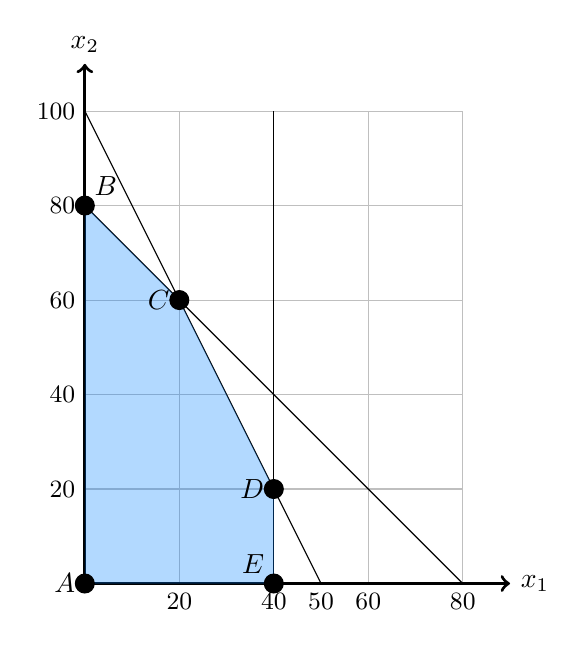
\begin{tikzpicture}[scale=0.06]
		\draw[gray!50, thin, step=20] (0,0) grid (80, 100);
		\draw[very thick,->] (0,0) -- (90, 0) node[right] {$x_1$};
		\draw[very thick,->] (0,0) -- (0, 110) node[above] {$x_2$};
		\foreach \x in {20,40,50,60,80} \draw (\x,0.05) -- (\x,-0.05) node[below] {\small\x};
		\foreach \y in {20,40,60,80,100} \draw (-0.05,\y) -- (0.05,\y) node[left] {\small\y};
		\draw (0,100) -- (50,0);
		\draw (0,80) -- (80,0);
		\draw (40,100) -- (40,0);
		\fill[blue!50!cyan,opacity=0.3] (0,0) -- (0,80) -- (20,60) -- (40,20) -- (40,0) -- cycle;
		\filldraw [black] (0,0) circle (2);
		\filldraw [black] (0,80) circle (2);
		\filldraw [black] (20,60) circle (2);
		\filldraw [black] (40,20) circle (2);
		\filldraw [black] (40,0) circle (2);
		\draw (0,0) node[left] {$A$};
		\draw (0,80) node[above right] {$B$};
		\draw (20,60) node[left] {$C$};
		\draw (40,20) node[left] {$D$};
		\draw (40,0) node[above left] {$E$};
	\end{tikzpicture}
	\caption[\textit{Corner points} pada daerah \textit{feasible}]{\textit{Corner points} pada daerah \textit{feasible}}
	\label{fig:corner_points}
\end{figure}

Tidak semua masalah \textit{linear programming} memiliki daerah \textit{feasible}. Apabila batasan-batasan dalam masalah tidak dapat membentuk daerah \textit{feasible}, maka masalah tersebut tidak memiliki solusi apapun, sehingga solusi optimal dari masalah tersebut tidak dapat dicari. Gambar~\ref{fig:daerah_infeasible} menunjukkan contoh masalah \textit{linear programming} yang tidak memiliki daerah \textit{feasible}.

\begin{figure}[H]
	\centering
	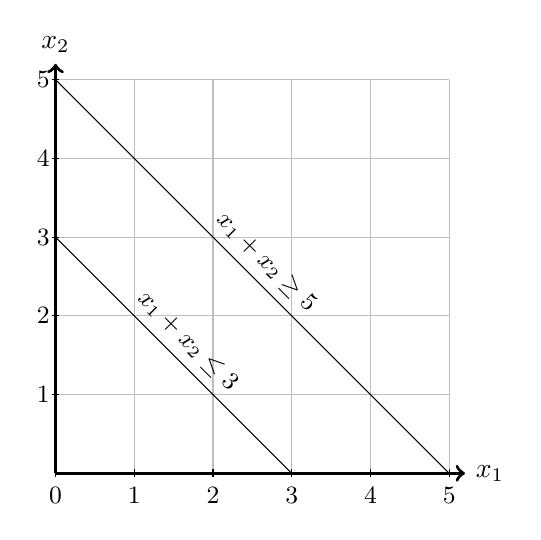
\begin{tikzpicture}
		\draw[gray!50, thin, step=1] (0,0) grid (5,5);
		\draw[very thick,->] (0,0) -- (5.2, 0) node[right] {$x_1$};
		\draw[very thick,->] (0,0) -- (0, 5.2) node[above] {$x_2$};
		\foreach \x in {0,...,5} \draw (\x,0.05) -- (\x,-0.05) node[below] {\small\x};
		\foreach \y in {1,...,5} \draw (-0.05,\y) -- (0.05,\y) node[left] {\small\y};
		\draw (3,0) -- node[above,sloped] {\small $x_1 + x_2 \leq 3$} (0,3);
		\draw (5,0) -- node[above,sloped] {\small $x_1 + x_2 \geq 5$} (0,5);
	\end{tikzpicture}
	\caption[Contoh masalah \textit{linear programming} tanpa daerah \textit{feasible}]{Contoh masalah \textit{linear programming} tanpa daerah \textit{feasible}}
	\label{fig:daerah_infeasible}
\end{figure}
	
%Batasan-batasan menghasilkan daerah solusi yang tidak tertutup. Daerah solusi ini memiliki jumlah solusi yang tak terhitung. Gambar~\ref{fig:daerah_solusi_tidak_dibatasi} berikut menggambarkan daerah solusi yang tidak dibatasi.
			
%    	\begin{figure}[H]
%    		\centering
%			\begin{tikzpicture}
%				\draw[gray!50, thin, step=1] (0,0) grid (5,5);
%				\draw[very thick,->] (0,0) -- (5.2, 0) node[right] {$x$};
%				\draw[very thick,->] (0,0) -- (0, 5.2) node[above] {$y$};
%				\foreach \x in {0,...,5} \draw (\x,0.05) -- (\x,-0.05) node[below] {\small\x};
%				\foreach \y in {1,...,5} \draw (-0.05,\y) -- (0.05,\y) node[left] {\small\y};
%				\draw (2,0) -- node[below,sloped] {\small $-2x + 3y \geq -4$} (5,2);
%				\draw (0,1) -- node[above,near end,sloped] {\small $4x - y \geq -1$} (1,5);
%				\fill[blue!50!cyan,opacity=0.3] (0,0) -- (0,1) -- (1,5) -- (5,5) -- (5,2) -- (2,0) -- cycle;
%			\end{tikzpicture}
%			\caption{Daerah solusi yang tidak dibatasi}
%			\label{fig:daerah_solusi_tidak_dibatasi}
%		\end{figure}

\subsection{Bentuk Standar}
Setiap masalah \textit{linear programming} harus diubah ke dalam bentuk standar sebelum diselesaikan. Berikut ini merupakan struktur dari bentuk standar pada masalah \textit{linear programming}:
    	
\begin{equation*}
	\setlength\arraycolsep{1.5pt}
	\begin{array}{r r c r c r c r c l}
	    \textit{max}		& \multicolumn{9}{l}{z = c_1x_1 + c_2x_2 + \dots + c_nx_n} \\
		\textit{s.t.} 	& a_{11}x_1 & + & a_{12}x_2 & + & \dots & + & a_{1n}x_n & = & b_1 \\
    						& a_{21}x_1 & + & a_{22}x_2 & + & \dots & + & a_{2n}x_n & = & b_2 \\
                            & \multicolumn{7}{c}{\vdots}                            &   & \vdots \\
                            & a_{m1}x_1 & + & a_{m2}x_2 & + & \dots & + & a_{mn}x_n & = & b_m \\
                            & \multicolumn{9}{l}{x_1\geq0,x_2\geq0,\dots,x_n\geq0}
	\end{array}
\end{equation*}

Bentuk standar masalah \textit{linear programming} terdiri dari $n$ buah variabel keputusan $x$ dan $m$ buah persamaan batasan. Setiap batasan dalam bentuk standar harus dalam bentuk persamaan dan batasan non-negatif diberlakukan untuk setiap varibel keputusan. Bentuk standar \textit{linear programming} dapat dinyatakan dalam notasi matriks seperti berikut ini:
        
\begin{equation*}
	\begin{array}{r l}
    	\textit{max}   & z=C^Tx \\
        \textit{s.t.} & Ax=b \textit{ and } x\geq0
	\end{array}    
\end{equation*}

dengan

%\begin{equation*}
%	c = \left[
%	\begin{array}{c}
%    	c_1\\
%    	c_2\\
%    	\vdots\\
%   	c_n
%	\end{array}
%	\right]    
%\end{equation*}

\begin{equation*}
	A = \left[
	\begin{array}{c c c c}
    	a_{11} & a_{12} & \dots & a_{1n}\\
    	a_{21} & a_{22} & \dots & a_{2n}\\
    	\vdots & \vdots & & \vdots\\
    	a_{m1} & a_{m2} & \dots & a_{mn}
	\end{array}
	\right]    
\end{equation*}

\begin{equation*}
	x = \left[
	\begin{array}{c}
    	x_1\\
    	x_2\\
    	\vdots\\
    	x_n
	\end{array}
	\right]    
\end{equation*}

\begin{equation*}
	b = \left[
	\begin{array}{c}
    	b_1\\
    	b_2\\
    	\vdots\\
    	b_m
	\end{array}
	\right]    
\end{equation*}

Pada notasi matriks, $x$ menunjukkan matriks kolom berdimensi $n$, $C^T$ menunjukkan matriks baris berdimensi $n$, $A$ menunjukkan matriks berdimensi $m\times n$, dan $b$ menunjukkan matriks kolom berdimensi $m$. Matriks $x\geq0$ menunjukkan batasan non-negatif untuk setiap variabel keputusan $x_i$. Untuk mengubah masalah \textit{linear programming} ke bentuk standar, maka setiap batasan perlu diubah. Perubahan batasan dibedakan berdasarkan tandanya, yaitu sebagai berikut:
		
		\begin{itemize}
			\item \textbf{Batasan dengan tanda pertidaksamaan \(\leq\)}\\
				Pertidaksamaan pada batasan ini diubah ke dalam bentuk persamaan dengan menambahkan variabel positif \(s_i\) yang disebut \textit{slack} pada sisi kiri. Lalu ditambahkan batasan non-negatif untuk variabel \textit{slack} tersebut. Contoh:
				
				\begin{equation*}
					x_1 + 2x_2 \leq 40
				\end{equation*}
				
				diubah menjadi
				
				\begin{equation*}
					\begin{split}
						x_1 + 2x_2 + s_1 &= 40\\
						s_1 &\geq 0
					\end{split}
				\end{equation*}
			
			\item \textbf{Batasan dengan tanda pertidaksamaan \(\geq\)}\\			
				Pertidaksamaan pada batasan ini diubah ke dalam bentuk persamaan dengan menambahkan variabel negatif \(e_i\) yang disebut \textit{excess} pada sisi kiri. Lalu ditambahkan batasan non-negatif untuk variabel \textit{excess} tersebut. Contoh:
				
				\begin{equation*}
					x_1 + 2x_2 \geq 40
				\end{equation*}
				
				diubah menjadi
				
				\begin{equation*}
					\begin{split}
						x_1 + 2x_2 - e_1 &= 40\\
						e_1 &\geq 0
					\end{split}
				\end{equation*}				
		\end{itemize}
		
%	\item Mengsubtitusi variabel bebas
	
%		Apabila terdapat variabel bebas \(x_i\), maka subtitusikan setiap variabel tersebut dengan 2 variabel pengganti \(u_i\) dan \(v_i\) sehingga \(x_i = u_i - v_i\). Lalu tambahkan tanda pembatas tidak negatif untuk variabel \(u_i\) dan \(v_i\). Contoh:
		
%		\begin{equation*}
%			\begin{array}{r r c r c l}
%				\text{maximize} & \multicolumn{5}{l}{z = x_1 + x_2}\\
%				\text{subject to} & 2x_1 & + & x_2 & \leq & 4\\
%									& \multicolumn{3}{r}{x_1} & \geq & 0\\
%			\end{array}
%		\end{equation*}
		
%		dengan
		
%		\begin{equation*}
%			x_2 = u_2 - v_2
%		\end{equation*}
		
%		menjadi
		
%		\begin{equation*}
%			\begin{array}{r r c r c r c l}
%				\text{maximize} & \multicolumn{7}{l}{z = x_1 + u_2 - v_2}\\
%				\text{subject to} & 2x_1 & + & u_2 & - & v_2 & \leq & 4\\
%									& \multicolumn{5}{r}{x_1} & \geq & 0\\
%									& \multicolumn{5}{r}{u_2} & \geq & 0\\
%									& \multicolumn{5}{r}{v_2} & \geq & 0\\
%			\end{array}
%		\end{equation*}
%\end{enumerate}

\subsection{Variabel Basis dan Non-basis}
Masalah \textit{linear programming} \(Ax = b\) terdiri dari \(m\) buah persamaan batasan dan \(n\) buah variabel keputusan. Masalah ini memiliki solusi yang disebut dengan solusi basis apabila membuat \((n - m)\) buah variabel keputusan bernilai 0 dan menyelesaikan \(m\) buah variabel keputusan lainnya. Sebanyak \((n - m)\) buah variabel yang dibuat bernilai 0 disebut dengan variabel non-basis. Sedangkan \(m\) buah variabel lainnya disebut dengan variabel basis. Berikut contoh sistem persamaan linear:
%Variabel basis merupakan variabel yang diselesaikan setelah membuat variabel lain menjadi variabel non basis. 

\begin{equation*}
	\setlength\arraycolsep{1.5pt}
	\begin{array}{r c r c r c l}
		x_1 &+ &x_2 &  &    &= &3\\
		    &- &x_2 &+ &x_3 &= &-1
	\end{array}
\end{equation*}

Pada sistem persamaan linear di atas, dipilih sebanyak 3 - 2 = 1 (3 variabel dan 2 persamaan) buah variabel yang akan menjadi variabel non basis. Jika himpunan variabel non basis NBV = \(\{x_3\}\), maka himpunan variabel basis BV = \(\{x_1, x_2\}\). Solusi dari sistem persamaan tersebut dapat dicari dengan membuat setiap variabel NBV menjadi variabel non basis dan menyelesaikan variabel BV.

\begin{equation*}
	\setlength\arraycolsep{1.5pt}
	\begin{array}{r c r c r c l}
		x_1 &+ &x_2 &  &    &= &3\\
		    &- &x_2 &+ &0 &= &-1
	\end{array}
\end{equation*}

Pada persamaan di atas didapatkan nilai \(x_1\) = 2 dan \(x_2\) = 1. Dengan demikian didapatkan solusi basis dengan nilai \(x_1\) = 2, \(x_2\) = 1, dan \(x_3\) = 0.

\subsection{Metode \textit{Simplex}}
Metode \textit{simplex} merupakan metode yang digunakan untuk menyelesaikan masalah \textit{linear programming}. Berikut ini merupakan langkah-langkah metode \textit{simplex}:
\begin{enumerate}
	\item Mengubah masalah \textit{linear programming} ke dalam bentuk standar.
	\item Mencari \textit{basic feasible solution} (\textit{bfs}) dari bentuk standar.
	\item Memeriksa apakah \textit{bfs} pada saat ini sudah optimal.
	\item Apabila \textit{bfs} belum optimal, tentukan variabel non-basis mana yang akan menjadi variabel basis dan tentukan variabel basis mana yang akan menjadi variabel non-basis dengan tujuan mencari \textit{bfs} baru yang dapat meningkatkan nilai fungsi objektif.
	\item Lakukan Operasi Baris Elementer (OBE) untuk mencari \textit{bfs} baru yang dapat meningkatkan nilai fungsi objektif. Lanjut ke langkah 3.
\end{enumerate}

Fungsi objektif yang berbentuk

\begin{equation*}
	z = c_1x_1 + c_2x_2 + \dots + c_nx_n
\end{equation*}

ditulis dalam bentuk

\begin{equation*}
	z - c_1x_1 - c_2x_2 - \dots - c_nx_n = 0
\end{equation*}

Bentuk fungsi objektif ini disebut sebagai baris 0.

Untuk memahami penyelesaian masalah \textit{linear programming} menggunakan metode \textit{simplex}, akan digunakan sebuah contoh masalah \textit{linear programming} sebagai berikut:

\begin{equation*}
	\setlength\arraycolsep{1.5pt}
	\begin{array}{r r c r c r c l}
		\textit{max } &\multicolumn{7}{l}{z = 60x_1 + 30x_2 + 20x_3}\\
		\textit{s.t.} &8x_1 &+ &6x_2 &+ &x_3 &\leq &48\\
		&4x_1 &+ &2x_2 &+ &1.5x_3 &\leq &20\\
		&2x_1 &+ &1.5x_2 &+ &0.5x_3 &\leq &8\\
		&&&x_2 &&&\leq &5\\
		&&&&&x_1 &\geq &0\\
		&&&&&x_2 &\geq &0\\
		&&&&&x_3 &\geq &0\\
	\end{array}
\end{equation*}

Langkah pertama adalah mengubah masalah ke bentuk standar, sehingga masalah ini dalam bentuk standar adalah sebagai berikut:

\begin{equation*}
	\setlength\arraycolsep{1.5pt}
	\begin{array}{r r c r c r c r c r c r c r c l}
		\textit{max } &\multicolumn{15}{l}{z = 60x_1 + 30x_2 + 20x_3}\\
		\textit{s.t.} &8x_1 &+ &6x_2 &+ &x_3 &+ &s_1 &&&&&&&= &48\\
		&4x_1 &+ &2x_2 &+ &1.5x_3 &&&+ &s_2 &&&&&= &20\\
		&2x_1 &+ &1.5x_2 &+ &0.5x_3 &&&&&+ &s_3 &&&= &8\\
		&&&x_2 && &&&&&&&+ &s_4 &= &5\\
		\multicolumn{14}{r}{x_1, x_2, x_3, s_1, s_2, s_3, s_4} &\geq &0\\
	\end{array}
\end{equation*}

Masalah dalam bentuk standar ini disajikan dalam bentuk tabel \textit{simplex} seperti pada tabel~\ref{tab:tabel_simplex_0}. Pada tabel ini, baris pertama (baris 0) merupakan baris bagi fungsi objektif dan baris lainnya merupakan baris bagi variabel basis. Pada tabel \textit{simplex} pertama, variabel basis terdiri dari variabel \textit{slack} dan variabel \textit{excess}.

\begin{center}
	\captionof{table}{Tabel \textit{simplex} 0}
	\label{tab:tabel_simplex_0}
	$
	\begin{array}{|r r r r r r r r|c|r c l|}
		\hline
		z & x_1 & x_2 & x_3 & s_1 & s_2 & s_3 & s_4 & \textit{rhs} & \multicolumn{3}{c|}{\textit{basic variable}}\\
		\hline
		1 & -60 & -30 & -20 & 0 & 0 & 0 & 0 & 0 & z & = & 0\\
		0 & 8 & 6 & 1 & 1 & 0 & 0 & 0 & 48 & s_1 & = & 48\\
		0 & 4 & 2 & 1.5 & 0 & 1 & 0 & 0 & 20 & s_2 & = & 20\\
		0 & 2 & 1.5 & 0.5 & 0 & 0 & 1 & 0 & 8 & s_3 & = & 8\\
		0 & 0 & 1 & 0 & 0 & 0 & 0 & 1 & 5 & s_4 & = & 5\\
		\hline
	\end{array}
	$
\end{center}

Kolom \textit{right hand side} (\textit{rhs}) menunjukkan nilai pada ruas kanan (nilai di sebelah kanan tanda sama dengan). Kolom \textit{basic variable} menunjukkan variabel basis beserta dengan nilainya. Kolom \textit{basic variable} juga menunjukkan solusi basis \textit{feasible} (\textit{bfs}) sehingga tabel~\ref{tab:tabel_simplex_0} menunjukkan \textit{bfs} dengan nilai \(z=0, x_1=0, x_2=0, x_3=0, s_1=48, s_2=20, s_3=8, \text{ dan } s_4=5\). Setiap variabel yang tidak berada di dalam kolom \textit{basic variable} menandakan bahwa variabel-variabel tersebut merupakan variabel non-basis sehingga bernilai 0.

Langkah selanjutnya adalah memeriksa apakah \textit{bfs} sudah optimal. Pada langkah ini akan diperiksa apakah terdapat variabel negatif (untuk kasus maksimasi) pada baris 0 di setiap kolom variabel. Pada tabel~\ref{tab:tabel_simplex_0}, masih terdapat variabel negatif, yaitu pada variabel \(x_1, x_2, \text{ dan } x_3\).
Hal ini menunjukkan bahwa \textit{bfs} saat ini masih belum optimal.

Apabila \textit{bfs} pada saat ini masih belum optimal, maka perlu dilakukan proses \textit{pivotting}. Proses \textit{pivotting} adalah proses penukaran variabel basis dengan variabel non-basis. Variabel yang akan menjadi variabel basis disebut dengan \textit{entering variable} dan variabel basis yang akan digantikan disebut dengan \textit{leaving variable}. \textit{Entering variable} dipilih dengan cara memilih variabel yang bernilai paling negatif pada baris 0. Untuk mencari \textit{leaving variable} perlu dilakukan tes rasio. Tes rasio membandingkan nilai pada nilai \textit{rhs} dengan nilai pada kolom \textit{entering variable}. Tes rasio hanya perlu dilakukan pada baris yang variable pada kolom \textit{entering variable} bernilai lebih besar dari 0. \textit{Leaving variable} dipilih dengan cara memilih variabel pada baris yang menghasilkan rasio terkecil. Perpotongan antara kolom \textit{entering variable} dengan baris \textit{leaving variable}.merupakan suatu elemen yang disebut \textit{pivot element}.

Dalam contoh masalah, \textit{bfs} pada saat ini masih belum optimal, sehingga perlu dilakukan proses \textit{pivotting}. Variabel \(x_1\) akan menjadi \textit{entering variable} karena bernilai paling negatif pada baris 0. Setelah dilakukan tes rasio sesuai, variabel \(s_3\) menjadi \textit{leaving variable} karena memiliki hasil tes rasio terkecil. Tes rasio untuk \textit{bfs} baru pada contoh masalah dapat dilihat pada tabel~\ref{tab:tabel_pivotting_1}.

\begin{center}
	\captionof{table}{Proses \textit{pivotting} 1}
	\label{tab:tabel_pivotting_1}
	$
	\begin{array}{|r r r r r r r r|c|r c l|r c l|}
		\hline
		z & x_1 & x_2 & x_3 & s_1 & s_2 & s_3 & s_4 & \textit{rhs} & \multicolumn{3}{c|}{\textit{basic variable}} & \multicolumn{3}{c|}{\textit{ratio}}\\
		\hline
		1 & -60 & -30 & -20 & 0 & 0 & 0 & 0 & 0 & z & = & 0 &&&\\
		0 & 8 & 6 & 1 & 1 & 0 & 0 & 0 & 48 & s_1 & = & 48 & \nicefrac{48}{8} & = & 6\\
		0 & 4 & 2 & 1.5 & 0 & 1 & 0 & 0 & 20 & s_2 & = & 20 & \nicefrac{20}{4} & = & 5\\
		0 & \encircle{2} & 1.5 & 0.5 & 0 & 0 & 1 & 0 & 8 & s_3 & = & 8 & \nicefrac{8}{2} & = & 4\\
		0 & 0 & 1 & 0 & 0 & 0 & 0 & 1 & 5 & s_4 & = & 5 &&&\\
		\hline
	\end{array}
	$
\end{center}

Setelah menentukan \textit{entering variable} dan \textit{leaving variable}, akan dilakukan Operasi Baris Elementer(OBE). OBE dilakukan untuk membuat \textit{entering variable} menjadi variabel basis, sehingga \textit{entering variable} pada baris {leaving variable} bernilai 1 dan variabel lain pada kolom \textit{entering variable} bernilai 0. Setelah OBE dilakukan, baris \textit{leaving variable} akan memiliki \textit{entering variable} sebagai variabel basis.

Dalam contoh masalah, telah ditentukan \textit{entering variable} dan \textit{leaving variable}. Variabel yang menjadi \textit{entering variable} adalah variabel \(x_1\) yang berada pada kolom \(x_1\). Variabel yang menjadi \textit{Leaving variable} adalah variabel \(s_3\) yang berada pada baris 3. Dengan OBE, \textit{entering variable} pada baris 3 akan dibuat bernilai 1 dan variabel lain pada kolom \textit{entering variable} akan dibuat bernilai 0. Berikut ini urutan OBE yang dilakukan:
\begin{enumerate}
	\item Untuk mendapatkan variabel \(x_1\) bernilai 1 pada baris 3, maka baris 3' baru dapat dibentuk dari baris 3 lama yang dikalikan dengan \(\nicefrac{1}{2}\).\\

	\begin{equation*}
		\frac{1}{2}R_3 \rightarrow R_3'
	\end{equation*}

	sehingga baris 3' baru menjadi

	\begin{equation*}
		x_1 + 0.75x_2 + 0.25x_3 + 0.5s_3 = 4
	\end{equation*}
	
	\item Untuk mendapatkan variabel \(x_1\) bernilai 0 pada baris 0, maka baris 0' baru dapat dibentuk dari baris 3' baru yang dikalikan 60 dan ditambahkan dengan baris 0 lama.\\

	\begin{equation*}
		60R_3 + R_0 \rightarrow R_0'
	\end{equation*}

	sehingga baris 0' baru menjadi

	\begin{equation*}
		z + 15x_2 - 5x_3 + 30s_3 = 240
	\end{equation*}

	\item Untuk mendapatkan variabel \(x_1\) bernilai 0 pada baris 1, maka baris 1' baru dapat dibentuk dari baris 3' baru yang dikalikan -8 dan ditambahkan dengan baris 1 lama.\\

	\begin{equation*}
		-8R_3 + R_1 \rightarrow R_1'
	\end{equation*}

	sehingga baris 1' baru menjadi

	\begin{equation*}
		-x_3 + s_1 - 4s_3 = 16
	\end{equation*}

	\item Untuk mendapatkan variabel \(x_1\) bernilai 0 pada baris 2, maka baris 2' baru dapat dibentuk dari baris 3' baru yang dikalikan -4 dan ditambahkan dengan baris 2 lama.\\

	\begin{equation*}
		-4R_2 + R_2 \rightarrow R_2'
	\end{equation*}

	sehingga baris 2' baru menjadi

	\begin{equation*}
		-x_2 + 0.5x_3 + s_2 - 2s_3 = 4
	\end{equation*}

\end{enumerate}

Karena nilai \(x_1\) bernilai 0 pada baris 4, maka tidak perlu dilakukan OBE pada baris 4, sehingga baris 4' baru sama dengan baris 4 lama. \textit{Entering variable} menggantikan \textit{leaving variable} pada baris 3 sehingga \(x_1\) menjadi variabel basis yang baru. Setelah melakukan OBE, maka didapatkan tabel \textit{simplex} baru seperti pada tabel~\ref{tab:tabel_simplex_1} yang menunjukkan \textit{bfs} dengan nilai \(z=240, x_1=4, x_2=0, x_3=0, s_1=16, s_2=4, s_3=0, \text{ dan } s_4=5\).

\begin{center}
	\captionof{table}{Tabel \textit{simplex} 1}
	\label{tab:tabel_simplex_1}
	$
	\begin{array}{|r r r r r r r r|c|r c l|}
		\hline
		z & x_1 & x_2 & x_3 & s_1 & s_2 & s_3 & s_4 & \textit{rhs} & \multicolumn{3}{c|}{\textit{basic variable}}\\
		\hline
		1 & 0 & 15 & -5 & 0 & 0 & 30 & 0 & 240 & z & = & 240\\
		0 & 0 & 0 & -1 & 1 & 0 & -4 & 0 & 16 & s_1 & = & 16\\
		0 & 0 & -1 & 0.5 & 0 & 1 & -2 & 0 & 4 & s_2 & = & 4\\
		0 & 1 & 0.75 & 0.25 & 0 & 0 & 0.5 & 0 & 4 & x_1 & = & 4\\
		0 & 0 & 1 & 0 & 0 & 0 & 0 & 1 & 5 & s_4 & = & 5\\
		\hline
	\end{array}
	$
\end{center}

Setelah mendapatkan tabel \textit{simplex}~\ref{tab:tabel_simplex_1}, langkah selanjutnya adalah memeriksa apakah \textit{bfs} pada iterasi ini sudah optimal. Pada baris 0, terdapat nilai negatif, yaitu pada variabel \(x_3\), sehingga \textit{bfs} ini belum optimal. Maka  langkah selanjutnya adalah mencari \textit{entering variable} dan \textit{leaving variable}. \textit{Entering variable} didapatkan dengan memilih variabel yang bernilai paling negatif pada baris 0, yaitu variabel \(x_3\). \textit{Leaving variable} didapatkan dengan mencari rasio terkecil dari hasil tes rasio. Tes rasio dapat dilihat pada tabel~\ref{tab:tabel_pivotting_2}. Variabel \(s_2\) menghasilkan hasil tes rasio terkecil, sehingga variabel \(s_2\) menjadi \textit{leaving variable}.

\begin{center}
	\captionof{table}{Proses \textit{pivotting} 2}
	\label{tab:tabel_pivotting_2}
	$
	\begin{array}{|r r r r r r r r|c|r c l|r c l|}
		\hline
		z & x_1 & x_2 & x_3 & s_1 & s_2 & s_3 & s_4 & \textit{rhs} & \multicolumn{3}{c|}{\textit{basic variable}} & \multicolumn{3}{c|}{\textit{ratio}}\\
		\hline
		1 & 0 & 15 & -5 & 0 & 0 & 30 & 0 & 240 & z & = & 240 &&&\\
		0 & 0 & 0 & -1 & 1 & 0 & -4 & 0 & 16 & s_1 & = & 16 &&&\\
		0 & 0 & -1 & \encircle{0.5} & 0 & 1 & -2 & 0 & 4 & s_2 & = & 4 & \nicefrac{4}{0.5} & = & 8\\
		0 & 1 & 0.75 & 0.25 & 0 & 0 & 0.5 & 0 & 4 & x_1 & = & 4 & \nicefrac{4}{0.25} & = & 16\\
		0 & 0 & 1 & 0 & 0 & 0 & 0 & 1 & 5 & s_4 & = & 5 &&&\\
		\hline
	\end{array}
	$
\end{center}

Selanjutnya dilakukan OBE untuk membuat \textit{entering variable} \(x_3\) menjadi variabel basis. Berikut ini urutan OBE yang dilakukan:
\begin{enumerate}
	\item Untuk mendapatkan variabel \(x_3\) bernilai 1 pada baris 2, maka baris 2'' baru dapat dibentuk dari baris 2' lama yang dikalikan dengan 2.\\

	\begin{equation*}
		2R_2' \rightarrow R_2''
	\end{equation*}

	sehingga baris 2'' baru menjadi

	\begin{equation*}
		-2x_2 + x_3 + 2s_2 - 4s_3 = 8
	\end{equation*}
	
	\item Untuk mendapatkan variabel \(x_3\) bernilai 0 pada baris 0, maka baris 0'' baru dapat dibentuk dari baris 2'' baru yang dikalikan 5 dan ditambahkan dengan baris 0' lama.\\

	\begin{equation*}
		5R_2'' + R_0' \rightarrow R_0''
	\end{equation*}

	sehingga baris 0'' baru menjadi

	\begin{equation*}
		z + 5x_2 + 10s_2 + 10s_3 = 280
	\end{equation*}
	
	\item Untuk mendapatkan variabel \(x_3\) bernilai 0 pada baris 1, maka baris 1'' baru dapat dibentuk dari baris 2'' baru yang ditambahkan dengan baris 1' lama.\\

	\begin{equation*}
		R_2'' + R_1' \rightarrow R_1''
	\end{equation*}

	sehingga baris 1'' baru menjadi

	\begin{equation*}
		-2x_2 + s_1 + 2s_2 - 8s_3 = 24
	\end{equation*}
	
	\item Untuk mendapatkan variabel \(x_3\) bernilai 0 pada baris 3, maka baris 3'' baru dapat dibentuk dari baris 2'' baru yang dikalikan \(-\nicefrac{1}{4}\) dan ditambahkan dengan baris 3' lama.\\

	\begin{equation*}
		-\frac{1}{4}R_2'' + R_3' \rightarrow R_3''
	\end{equation*}

	sehingga baris 3'' baru menjadi

	\begin{equation*}
		x_1 + 1.25x_2 - 0.5s_2 + 1.5s_3 = 2
	\end{equation*}
\end{enumerate}

Variabel \(x_3\) sudah bernilai 0 pada baris 4, maka baris 4 yang baru sama dengan baris 4 yang lama. Variabel \(x_3\) menjadi variabel basis baru yang menggantikan variabel \(s_2\). Setelah melakukan OBE, didapatkan tabel \textit{simplex}~\ref{tab:tabel_simplex_2} yang menunjukkan \textit{bfs} dengan nilai \(z=280, x_1=2, x_2=0, x_3=8, s_1=24, s_2=0, s_3=0, \text{ dan } s_4=5\).

\begin{center}
	\captionof{table}{Tabel \textit{simplex} 2}
	\label{tab:tabel_simplex_2}
	$
	\begin{array}{|r r r r r r r r|c|r c l|}
		\hline
		z & x_1 & x_2 & x_3 & s_1 & s_2 & s_3 & s_4 & \textit{rhs} & \multicolumn{3}{c|}{\textit{basic variable}}\\
		\hline
		1 & 0 & 5 & 0 & 0 & 10 & 10 & 0 & 280 & z & = & 280\\
		0 & 0 & -2 & 0 & 1 & 2 & -8 & 0 & 24 & s_1 & = & 24\\
		0 & 0 & -2 & 1 & 0 & 2 & -4 & 0 & 8 & x_3 & = & 8\\
		0 & 1 & 1.25 & 0 & 0 & -0.5 & 1.5 & 0 & 2 & x_1 & = & 2\\
		0 & 0 & 1 & 0 & 0 & 0 & 0 & 1 & 5 & s_4 & = & 5\\
		\hline
	\end{array}
	$
\end{center}

Langkah selanjutnya adalah memeriksa apakah \textit{bfs} saat ini sudah optimal. Pada baris 0, tidak ditemukan variabel bernilai negatif, sehingga \textit{bfs} pada tahap ini sudah optimal. Dengan demikian masalah ini memiliki solusi optimal bernilai 280 dengan variabel \(x_1=2, x_2=0, x_3=8, \text{ dan } x_4 = 0\).

Contoh yang dibahas sebelumnya merupakan contoh masalah \textit{linear programming} dalam kasus maksimisasi. Untuk menyelesaikan masalah \textit{linear programming} pada kasus minimasi, dapat dilakukan dengan mengubah tujuan minimasi menjadi tujuan maksimasi. Perubahan tujuan ini dilakukan dengan mengalikan fungsi tujuan dengan -1. Contoh:

\begin{equation*}
	\setlength\arraycolsep{1.5pt}
	\begin{array}{r r c r c l}
		\textit{min } &\multicolumn{5}{l}{z = 2x_1 - 3x_2}\\
		\textit{s.t.} &x_1 &+ &x_2 &\leq &4\\
		&x_1 &- &x_2 &\leq &6\\
		&&&x_1 &\geq &0\\
		&&&x_2 &\geq &0\\
	\end{array}
\end{equation*}

Contoh tersebut merupakan contoh masalah \textit{linaer programming} dengan tujuan minimasi. Untuk menyelesaikannya, fungsi objektif dikalikan dengan -1, sehingga tujuan berubah menjadi maksimasi. Contoh masalah berubah menjadi:

\begin{equation*}
	\setlength\arraycolsep{1.5pt}
	\begin{array}{r r c r c l}
		\textit{max } &\multicolumn{5}{l}{-z = -2x_1 + 3x_2}\\
		\textit{s.t.} &x_1 &+ &x_2 &\leq &4\\
		&x_1 &- &x_2 &\leq &6\\
		&&&x_1 &\geq &0\\
		&&&x_2 &\geq &0\\
	\end{array}
\end{equation*}

Tabel~\ref{tab:tabel_simplex_minimasi_0} menunjukkan tabel \textit{simplex} awal untuk contoh masalah \textit{linear programming} kasus minimasi. Tabel~\ref{tab:tabel_simplex_minimasi_1} menunjukkan tabel \textit{simplex} yang menghasilkan \textit{bfs} optimal dengan nilai \(-z=12, x_1=0, x_2=4, s_1=0, \text{ dan } s_2=10\). Dengan demikian, didapatkan solusi optimal sebesar -12 dengan variabel \(x_1=0 \text{ dan } x_2=4\).

\begin{center}
	\captionof{table}{Tabel \textit{simplex} 0 untuk kasus minimasi}
	\label{tab:tabel_simplex_minimasi_0}
	$
	\begin{array}{|r r r r r |c|r c l|r c l|}
		\hline
		-z & x_1 & x_2 & s_1 & s_2 & \textit{rhs} & \multicolumn{3}{c|}{\textit{basic variable}} & \multicolumn{3}{c|}{\textit{ratio}}\\
		\hline
		1 & 2 & -3 & 0 & 0 & 0 & -z & = & 0 &&&\\
		0 & 1 & \encircle{1} & 1 & 0 & 4 & s_1 & = & 4 & \nicefrac{4}{1} & = & 4\\
		0 & 1 & -1 & 0 & 1 & 6 & s_2 & = & 6 &&&\\
		\hline
	\end{array}
	$
\end{center}

\begin{center}
	\captionof{table}{Tabel \textit{simplex} 1 untuk kasus minimasi}
	\label{tab:tabel_simplex_minimasi_1}
	$
	\begin{array}{|r r r r r |c|r c l|}
		\hline
		-z & x_1 & x_2 & s_1 & s_2 & \textit{rhs} & \multicolumn{3}{c|}{\textit{basic variable}}\\
		\hline
		1 & 5 & 0 & 3 & 0 & 12 & -z & = & 12\\
		0 & 1 & 1 & 1 & 0 & 4 & x_2 & = & 4\\
		0 & 2 & 0 & 1 & 1 & 10 & s_2 & = & 10\\
		\hline
	\end{array}
	$
\end{center}

%\section{Integer Programming}
%
%Integer programming merupakan teknik lanjutan dari linear programming di mana setiap variabel pada solusi optimal harus berupa bilangan bulat~\cite{winston2004operations}. Terdapat beberapa metode yang dapat digunakan untuk menyelesaikan masalah integer programming, salah satunya adalah metode \textit{branch and bound}.
%
%\subsection{Metode \textit{Branch and Bound}}
%\textit{Branch and bound} merupakan metode penyelesaian masalah integer programming dengan memecah masalah menjadi sub-sub masalah. Pemecahan masalah akan terus dilakukan hingga didapatkan solusi optimal yang terdiri dari variabel berupa bilangan bulat. Berikut langkah-langkah metode \textit{branch and bound}:
%
%\begin{enumerate}
%	\item Selesaikan masalah menggunakan metode simplex. Apabila solusi optimal yang didapatkan terdiri dari variabel berupa bilangan bulat, maka proses berhenti pada tahap ini. Solusi ini menjadi solusi optimal dalam permasalahan ini. Apabila sebaliknya, maka dilanjutkan ke tahap selanjutnya. Solusi pada tahap ini akan menjadi solusi batas atas yang akan digunakan sebagai pembanding di tahap-tahap selanjutnya.
%
%	\item Tentukan satu variabel yang nilainya pada solusi tidak berupa bilangan bulat. Variabel ini akan menjadi variabel terpilih yang akan digunakan di tahap selanjutnya.
%
%	\item Buat 2 sub masalah baru. Sub-sub masalah tersebut merupakan masalah yang sama dengan adanya sebuah tambahan batasan baru. 
%	\begin{enumerate}
%		\item Sub masalah pertama memiliki tambahan batasan baru yang menyatakan bahwa variabel terpilih harus bernilai lebih kecil atau sama dengan pembulatan ke bawah dari nilai variabel terpilih.
%		
%		\item Sub masalah kedua memiliki tambahan batasan baru yang menyatakan bahwa variabel terpilih harus bernilai lebih besar atau sama dengan pembulatan ke atas dari nilai variabel terpilih.
%	\end{enumerate}
%		
%	\item Selesaikan setiap sub masalah menggunakan metode simplex dan periksa solusinya.
%	\begin{enumerate}
%		\item Apabila setiap variabel pada solusi berupa bilangan bulat, maka bandingkan solusi ini dengan solusi batas atas. Apabila solusi ini sama dengan batas atas, maka solusi ini merupakan solusi optimal dalam permasalahan ini dan proses berhenti pada tahap ini. Apabila solusi lebih buruk dari solusi batas atas, maka bandingkan dengan solusi batas bawah. Apabila solusi ini lebih baik daripada solusi batas bawah, maka jadikanlah solusi ini sebagai solusi batas bawah yang baru.
%		
%		\item Apabila setiap variabel pada solusi tidak berupa bilangan bulat, maka periksa apakah solusi ini lebih baik daripada solusi batas bawah. Apabila lebih baik, maka dilanjukan pada tahap ke-2 untuk memecah sub masalah ini. Apabila tidak lebih baik, maka sub masalah ini tidak perlu dipecah lagi karena tidak akan menghasilkan solusi yang lebih baik.
%		
%		\item Apabila sub masalah tidak dapat diselesaikan (\textit{infeasible}), maka sub masalah ini tidak perlu dilanjutkan lagi.		
%	\end{enumerate}
%\end{enumerate}

\section{\textit{Binary Integer Programming}}
\label{sec:bip}
\textit{Binary integer programming} adalah lanjutan dari linear programming di mana setiap variabel keputusan pada solusi optimal harus bernilai 0 atau 1. Bentuk umum masalah \textit{binary integer programming} adalah seperti berikut:

\begin{equation}
\begin{array}{r l}
\textit{min}   & z=C^Tx \\
\textit{s.t.} & Ax\geq b \\
& x \in \{0,1\}
\end{array}    
\end{equation}

Terdapat sebuah algoritma yang diciptakan oleh Egon Balas~\cite{balas1965additive} bernama \textit{Balas's additive} yang digunakan untuk menyelesaikan masalah \textit{binary integer programming}. Algoritma \textit{Balas's additive} akan dibahas lebih lanjut pada~\ref{balas_additive}.

\subsection{Algoritma \textit{Balas's Additive}}
\label{balas_additive}
Setiap masalah \textit{binary integer programming} memiliki kemungkinan solusi berjumlah \(2^n\) karena setiap variabel hanya dapat bernilai 0 atau 1 saja. Apabila menggunakan algoritma \textit{Balas's additive}, maka solusi optimal dari masalah \textit{binary integer programming} pada umumnya (\textit{average case}) dapat ditemukan tanpa perlu memeriksa seluruh \(2^n\) kemungkinan. Dengan demikian, algoritma \textit{Balas's additive} dapat digunakan untuk menemukan solusi optimal bagi masalah \textit{binary integer programming} secara efisien.

Untuk menyelesaikan masalah \textit{binary integer programming} menggunakan algoritma \textit{Balas's additive}, maka masalah perlu diubah terlebih dahulu berdasarkan ketentuan-ketentuan berikut ini:

\begin{itemize}
	\item Fungsi tujuan dinyatakan dalam bentuk \textit{min} \(z=\sum_{j=1}^{n}c_jx_j\).
	\item Sebanyak \(m\) batasan harus dinyatakan dalam bentuk pertidaksamaan \(\sum a_{ij} x_j\geq b_i\) untuk \(i=1,2,\dots,m\).
	\item Setiap variabel \(x_j\) dimana \(j=1,2,\dots,n\) harus merupakan variabel biner (variabel yang hanya dapat bernilai 0 atau 1).
	\item Koefisien dari setiap varibel pada fungsi tujuan tidak bernilai negatif.
	\item Setiap variabel pada fungsi tujuan diurutkan menaik berdasarkan koefisiennya sehingga \(0\leq c_1 \leq c_2 \leq \dots \leq c_n\).
\end{itemize}

Pengurutan variabel secara menaik berdasarkan koefisiennya bertujuan agar nilai \(z\) meningkat dengan nilai seminimum mungkin pada setiap iterasi. Mulanya algoritma \textit{Balas's additive} akan membuat seluruh variabel bernilai 0 agar mendapatkan nilai \(z\) yang paling minimum. Apabila solusi bersifat \textit{infeasible}, maka algoritma akan memilih variabel dengan indeks yang terdekat dengan 1 untuk bernilai 1. Hal ini akan menyebabkan nilai \(z\) meningkat dengan nilai terkecil karena variabel telah terurut menaik berdasarkan koefisiennya.

Algoritma \textit{Balas's additive} menggunakan paradigma algoritma \textit{branch and bound}~\cite{narendra1977branch} untuk mendapatkan solusi optimal dari seluruh kemungkinan solusi yang ada. \textit{Branch and bound} merupakan algoritma yang dapat mencari solusi terbaik dari suatu himpunan solusi tanpa melibatkan \textit{exhaustive search}. \textit{Branch and bound} bekerja dengan cara dengan membagi himpunan solusi menjadi beberapa subhimpunan secara rekursi hingga mendapatkan solusi terbaik. Pembagian ini hanya dilakukan pada setiap subhimpunan yang dapat menghasilkan solusi terbaik. \textit{Branch and bound} menggunakan struktur data \textit{tree} di mana \textit{root} menunjukkan himpunan keseluruhan solusi dan cabang menunjukkan subhimpunannya. Terdapat 2 proses utama dalam \textit{branch and bound}, yaitu \textit{branching} dan \textit{bounding}. \textit{Branching} berfungsi untuk membagi himpunan solusi menjadi beberapa subhimpunan yang lebih kecil. \textit{Bounding} berfungsi untuk menetapkan nilai \textit{bound} bagi suatu subhimpunan. Nilai \textit{bound} merupakan nilai pembanding dalam menentukan subhimpunan mana yang akan dibagi.

\textit{Branch and bound} pada algoritma \textit{Balas's additive} dilakukan dengan menggunakan struktur data \textit{binary tree} karena setiap percabangan menghasilkan 2 \textit{node} di mana salah satu node menunjukkan variabel bernilai 0 dan node lainnya menunjukkan variabel bernilai 1. Setiap tingkat kedalaman pada \textit{binary tree} mengacu pada setiap variabel sesuai dengan urutan yang telah dilakukan sebelumnya. \textit{Branching} terhadap suatu \textit{node} akan menghasilkan 2 \textit{node} baru, yaitu \textit{node} \(x_N=0\) dan \textit{node} \(x_N=1\) di mana \(x_N\) merupakan variabel \(x\) \textit{now} (\(x\) yang diacu oleh \textit{node} pada saat ini) bukan variabel \(x_n\) (\(x\) terakhir dalam kumpulan \(x\)). \textit{Bounding} pada algoritma \textit{Balas's additive} dibedakan menjadi 2 berdasarkan nilai \(x_N\), yaitu:

\begin{itemize}
	\item Apabila \(x_N = 1\), maka algoritma berasumsi bahwa \textit{node} pada saat ini dapat menghasilkan solusi \textit{feasible} sehingga nilai \textit{bound} untuk \textit{node} ini adalah \(\sum_{j=1}^{N} c_j x_j\). Karena variabel telah diurutkan sebelumnya, maka nilai \textit{bound} ini dipastikan menjadi yang paling rendah untuk saat ini.
	
	\item Apabila \(x_N = 0\), maka nilai \textit{bound} dari \textit{node} ini adalah \(\sum_{j=1}^{N} c_j x_j + c_{N+1}\). \textit{Node} ini terbentuk karena \textit{node} sebelumnya memiliki solusi yang bersifat \textit{infeasible}. Hal tersebut disebabkan oleh adanya batasan \(\geq\) yang tidak terpenuhi karena total ruas kiri yang lebih kecil daripada ruas kanan. Apabila variabel saat ini bernilai 0, maka batasan tersebut tetap tidak akan terpenuhi sehingga setidaknya harus terdapat 1 variabel lainnya yang bernilai 1, yaitu \(x_{N+1}\). Variabel tersebut dipilih untuk memastikan bahwa nilai \textit{bound} pada saat ini merupakan yang paling rendah.
\end{itemize}

Setiap node menunjukkan solusi yang belum tentu bersifat \textit{feasible} sehingga perlu dilakukannya pengecekan. Untuk menentukan apakah solusi bersifat \textit{feasible}, maka akan diasumsikan bahwa variabel setelah \(x_N\) (saat \(x_N=1\)) atau \(x_{N+1}\) (saat \(x_N=0\)) bernilai 0. Selanjutnya, solusi ini akan diuji terhadap setiap batasan. Apabila tidak terdapat batasan yang dilanggar, maka solusi bersifat \textit{feasible} dan \textit{node} dinyatakan \textit{fathomed} sehingga tidak perlu dilakukan \textit{branching}. \textit{Branching} tidak perlu dilakukan karena turunannya tidak akan menghasilkan solusi yang lebih baik. Hal ini telah dipastikan ketika melakukan proses \textit{bounding}. Solusi \textit{feasible} ini kemudian dibandingkan dengan \textit{incumbent} yang telah ditemukan sebelumnya. Apabila lebih baik, maka solusi ini menjadi \textit{incumbent} yang baru. Apabila \textit{node} memiliki solusi yang bersifat \textit{infeasible}, maka akan dilakukan \textit{branching}. Namun sebelum melakukan \textit{branching}, akan dilakukan pengecekan untuk mengetahui apakah turunan dari \textit{node} dapat menghasilkan solusi \textit{feasible}. Pengecekan dilakukan dengan memastikan bahwa setiap batasan memiliki kemungkinan untuk dipenuhi, yaitu dengan memastikan bahwa ruas kiri dengan kemungkinan variabel tersisanya dapat menghasilkan total yang tidak lebih kecil daripada ruas kanan. Total ruas kiri terbesar dapat dicari dengan menjumlahkan ruas kiri untuk variabel hingga saat ini dengan total nilai koefisien positif untuk variabel tersisa. Apabila terdapat 1 atau lebih batasan di mana total ruas kiri lebih kecil daripada nilai ruas kanan, maka \textit{node} tersebut dinyatakan \textit{fathomed} sehingga tidak perlu dilakukan \textit{branching}. \textit{Branching} tidak perlu dilakukan karena batasan tidak dapat dipenuhi dengan berapa pun nilai dari variabel tersisa. Apabila setiap batasan memiliki kemungkinan untuk dipenuhi, maka akan dilakukan \textit{branching} pada \textit{node} tersebut.

%\section{Kakas \textit{lp{\_}solve}}
%Kakas \textit{lp{\_}solve} merupakan kakas perangkat lunak yang berguna untuk menyelesaikan masalah linear programming\footnote{http://lpsolve.sourceforge.net/5.5/}. Kakas ini dapat menerima masalah linear programming atau masalah integer programming. Kakas lp{\_}solve menggunakan metode \textit{branch and bound} untuk menyelesaikan masalah integer programming. Kakas ini dibangun dengan bahasa pemrograman ANSI C yang dapat dikompilasi dalam lingkungan Unix dan Windows. Untuk menggunakan kakas lp{\_}solve dalam lingkungan pemrograman Java, kakas lp{\_}solve menyediakan kakas penghubung dalam bahasa pemrograman Java sehingga aplikasi Java dapat menggunakan kakas lp{\_}solve. Berikut ini merupakan contoh penggunaan kakas lp{\_}solve dalam pemrograman Java:
%\begin{lstlisting}[language=Java, caption=Demo.java]
%import lpsolve.*;
%
%public class Demo {
%
%  public static void main(String[] args) {
%    try {
%      // Create a problem with 4 variables and 0 constraints
%      LpSolve solver = LpSolve.makeLp(0, 4);
%
%      // add constraints
%      solver.strAddConstraint("3 2 2 1", LpSolve.LE, 4);
%      solver.strAddConstraint("0 4 3 1", LpSolve.GE, 3);
%
%      // set objective function
%      solver.strSetObjFn("2 3 -2 3");
%
%      // solve the problem
%      solver.solve();
%
%      // print solution
%      System.out.println("Value of objective function: " 
%        + solver.getObjective());
%      double[] var = solver.getPtrVariables();
%      for (int i = 0; i < var.length; i++) {
%        System.out.println("Value of var[" + i + "] = " + var[i]);
%      }
%
%      // delete the problem and free memory
%      solver.deleteLp();
%    }
%    catch (LpSolveException e) {
%       e.printStackTrace();
%    }
%  }
%}
%\end{lstlisting}

\section{Penelitian Terkait}
Penelitian untuk mencari penempatan sensor visual secara optimal telah dilakukan sebelumnya oleh Horster dan Lienhart~\cite{horster2006approximating}. Masalah yang dibahas penelitian ini adalah cara menentukan jumlah sensor visual minimum beserta dengan lokasi penempatan dan arah pandangnya. Masalah ini dibatasi pada bidang 2D dan ruangan yang digunakan diasumsikan berbentuk persegi panjang.

Daerah cakupan kamera berbentuk segitiga seperti pada gambar~\ref{fig:fieldofviewhorster}.
\begin{figure}[H]
	\centering
	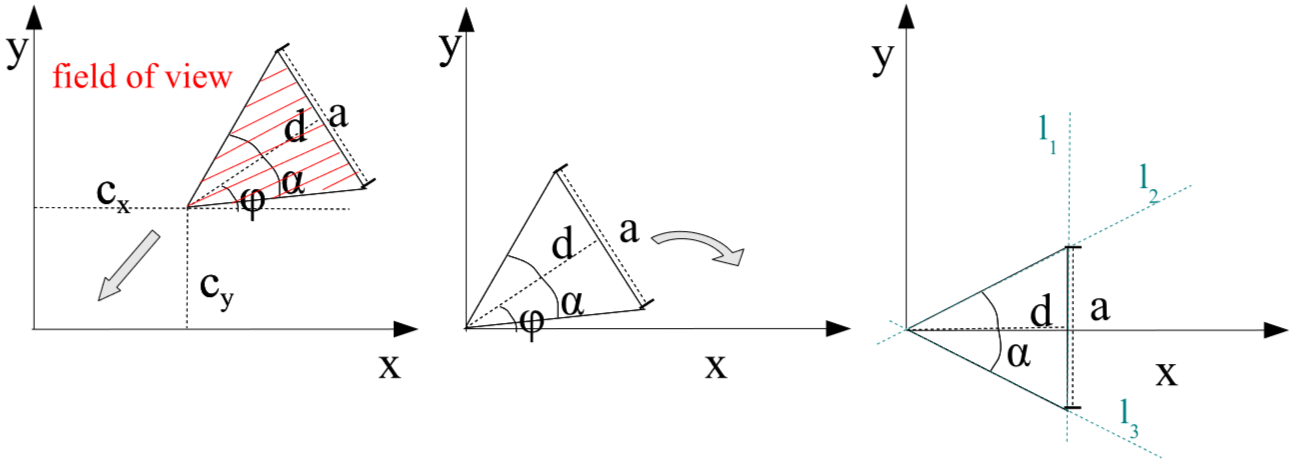
\includegraphics[scale=0.4]{fieldofviewhorster}
	\caption[Pemodelan daerah cakupan kamera]{Pemodelan daerah cakupan kamera}
	\label{fig:fieldofviewhorster}
\end{figure}
Kamera ditempatkan pada posisi \(c_x,x_y\) dan menghadap ke arah \(\varphi\). Untuk mendapatkan daerah cakupan kamera, mulanya kamera ditranslasi ke titik \textit{origin} pada sistem koordinat:
\begin{equation}
	x'=x-c_x
\end{equation}
\begin{equation}
	y'=y-c_y
\end{equation}
Selanjutnya, daerah cakupan diputar sehingga sumbu pandang menjadi paralel terhadap sumbu x:
\begin{equation}
	x''=\cos(\varphi)\cdot x'+\sin(\varphi)\cdot y'
\end{equation}
\begin{equation}
	y''=-\sin(\varphi)\cdot x'+\cos(\varphi)\cdot y'
\end{equation}
Daerah cakupan kamera dapat ditentukan dengan garis \(l_1,l_2,l_3\):
\begin{equation}
	l_1:x''\leq d
\end{equation}
\begin{equation}
	l_2:y''\leq \frac{a}{2d}\cdot x''
\end{equation}
\begin{equation}
	l_3:y''\geq-\frac{a}{2d}\cdot x''
\end{equation}
Dengan subtitusi, didapatkan daerah cakupan kamera berdasarkan tiga persamaan berikut ini:
\begin{equation}
	\cos(\varphi)\cdot(x-c_x)+\sin(\varphi)\cdot(y-c_y)'\leq d
	\label{eq:l1}
\end{equation}
\begin{equation}
	-\sin(\varphi)\cdot(x-c_x)+\cos(\varphi)\cdot(y-c_y)\leq \frac{a}{2d}\cdot (\cos(\varphi)\cdot(x-c_x)+\sin(\varphi)\cdot(y-c_y))	\label{eq:l2}
\end{equation}
\begin{equation}
	-\sin(\varphi)\cdot(x-c_x)+\cos(\varphi)\cdot(y-c_y)\geq- \frac{a}{2d}\cdot (\cos(\varphi)\cdot(x-c_x)+\sin(\varphi)\cdot(y-c_y))
	\label{eq:l3}
\end{equation}

Ruangan dimodelkan dengan membentuk \textit{grid points} 2 dimensi dengan jarak antar titik sebesar \(f_a\). Kamera hanya dapat diletakkan pada titik dalam \textit{grid point} dan cakupan kamera hanya periksa terhadap titik dalam \textit{grid point}. Ruangan berbentuk persegi panjang terdiri dari ukuran lebar \(w\) dan tinggi \(h\) tanpa penghalang apapun di dalamnya.

Titik penempatan kamera dinyatakan dalam himpunan \(s_x\) dan himpunan \(s_y\) sesuai dengan dimensi \(x-\) dan \(y-\) pada \textit{grid point}. Selain itu, terdapat himpunan \(s_\varphi\) yang menyatakan arah pandang yang memungkinkan bagi setiap kamera. Kamera yang ditempatkan pada (\(c_x,c_y\)) dengan arah pandang \(\varphi\) dapat mencakup \textit{grid point} (\(x,y\)) jika dan hanya jika persamaan~\ref{eq:l1},~\ref{eq:l2}, dan~\ref{eq:l3} terpenuhi.

Masalah dimodelkan ke dalam bentuk \textit{linear programming} dengan tujuan mendapatkan jumlah kamera minimum berdasarkan \textit{grid point} dan model kamera yang diberikan dengan tetap memastikan bahwa setiap titik pada \textit{grid point} tercakup oleh setidaknya satu kamera. Variabel biner \(x_{ij\varphi}\) didefinisikan sebagai berikut:
\begin{equation}
	x_{ij\varphi}=\left\{
		\begin{array}{cl}
			1 & \text{jika kamera yang ditempatkan pada \textit{grid point} }(i,j)\\\\
			0 & \text{jika sebaliknya}
		\end{array}
	\right.
\end{equation}
Total kamera \(N\) didapatkan dengan:
\begin{equation}
	N=\sum_{\varphi=0}^{s_\varphi-1}\sum_{i=0}^{s_i-1}\sum_{j=0}^{s_j-1}x_{ij\varphi}
\end{equation}
Untuk menentukan ketercakupan titik, dibentuk fungsi biner \(c(i1,j1,\varphi1,i2,j2)\):
\begin{equation}
	c(i1,j1,\varphi1,i2,j2)=\left \{
		\begin{array}{cl}
			1 & \text{jika kamera yang ditempatkan pada \textit{grid point} }(i1,j1)\\
			 & \text{dengan arah pandang }\varphi{1}\text{ dapat mencakup \textit{grid point} }(i2,j2)\\\\
			 0 & \text{jika sebaliknya}
		\end{array}
	\right.
\end{equation}
Dengan demikian masalah dapat diformulasikan ke dalam bentuk \textit{linear programming} sebagai berikut:
\begin{equation}
	\begin{split}
		\textit{min } & \sum_{\varphi=0}^{s_\varphi-1}\sum_{i=0}^{s_i-1}\sum_{j=0}^{s_j-1}x_{ij\varphi}\\
		\textit{s.t. } & \sum_{\varphi{1}=0}^{s_\varphi-1}\sum_{i1=0}^{s_i-1}\sum_{j1=0}^{s_j-1}x_{i1,j1,\varphi{1}}\cdot c(i1,j1,\varphi1,i2,j2)\geq 1\\
		&0\leq i2\leq(s_x-1), 0\leq j2\leq(s_y-1)
	\end{split}
	\label{eq:lpformhorster}
\end{equation}
Batasan pada~\ref{eq:lpformhorster} memastikan bahwa setiap titik pada \textit{grid point} akan dicakup oleh setidaknya 1 kamera. Untuk memastikan bahwa hanya terdapat maksimal 1 kamera yang dapat ditempatkan pada setiap titik, maka dapat ditambahkan batasan berikut ini:
\begin{equation}
	\begin{split}
		\sum_{\varphi=0}^{s_\varphi-1}x_{ij\varphi}&\leq 1\\
		0\leq i\leq(s_x-1), 0&\leq j\leq(s_y-1)
	\end{split}
\end{equation}
Jumlah variabel \(x_{ij\varphi}\) dalam model \textit{linear programing} ini adalah sebesar \(s_x\cdot s_y\cdot s_\varphi\). Jika ukuran \textit{grid point} diperbesar, maka jumlah variabel dan batasan pada model \textit{linear programming} juga akan semakin besar. Karena variabel yang digunakan bersifat biner, maka masalah \textit{linear programming} ini dapat diselesaikan menggunakan teknik \textit{binary integer programming}~\ref{sec:bip}.